%\chapter*{Anhang}

\pagenumbering{Roman}

\appendix

\chapter{Ausschreibung Bachelorarbeit}\label{anhang_ausschreibung} 


\chapter{Projektplanung}\label{anhang_projektplan} 

\chapter{Referenz Sensortag von Texas Instrument}\label{anhang_sensortag} 
Im Rahmen dieser Bachelorarbeit sind nicht Microcontroller für Low Power Anwendungen zu evaluieren. Das Sensortag von Texax Instrument ist vorgegeben und beinhaltet für die Entwicklung des Bicycle Computer bereits mehrere Eigenschaften auf einem Borad vereint:

\begin{itemize}
    \item Bestückt mit 10 Sensoren
    \item Bestückt mit einem zweiten Cortex für die Wireless-Anbindung.
          Dadurch leichtes Wechseln der Kommunikationsart von Bluetooth smart auf z.B. Zigbee.
    \item Hohe Rechenleistung
\end{itemize}


\section{Blockschema Sensortag}


\begin{figure}
    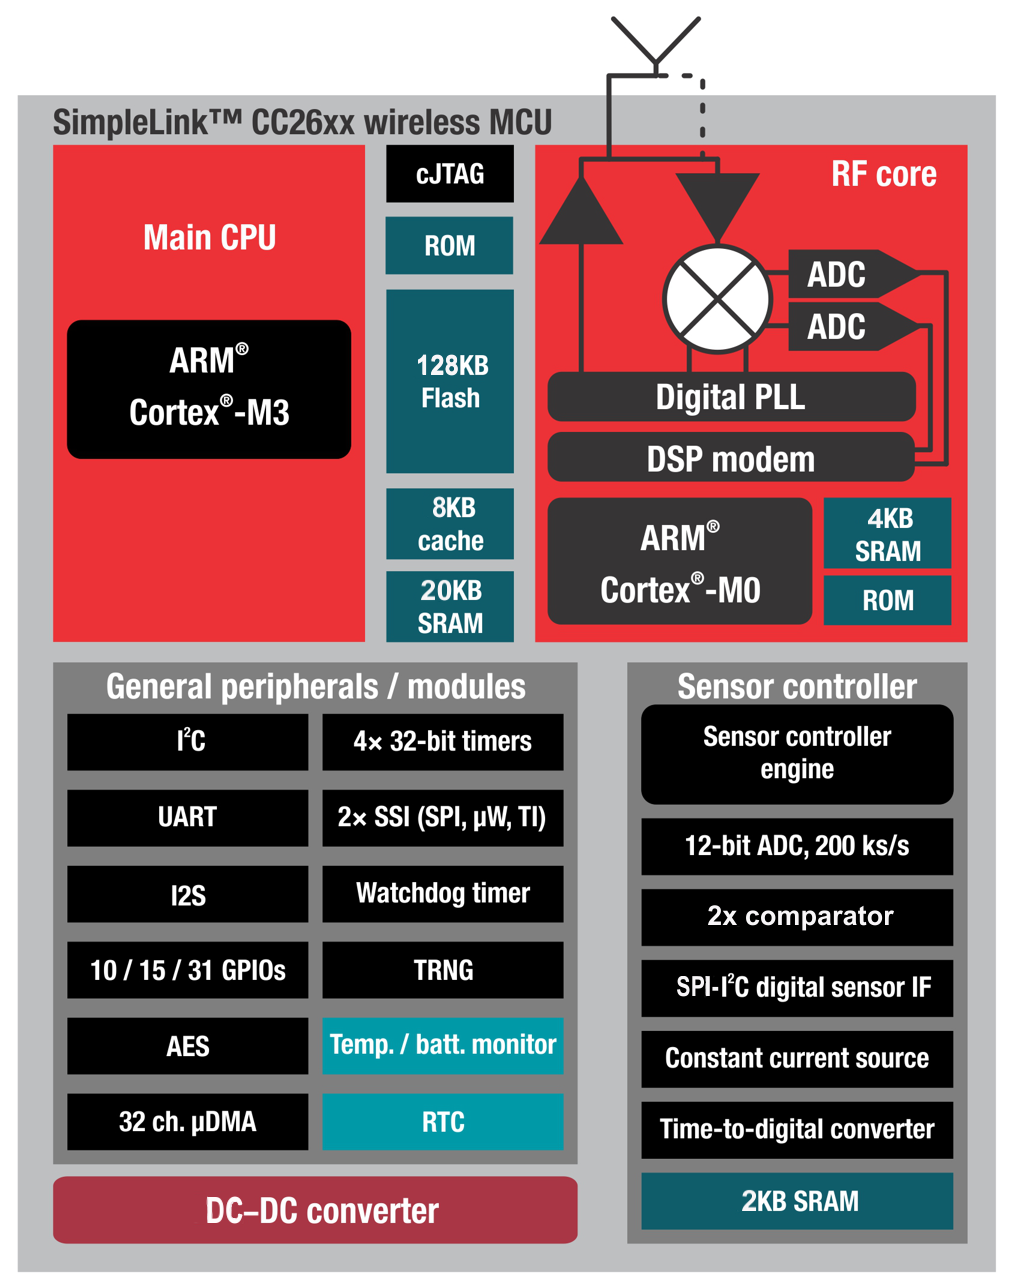
\includegraphics[scale=1]{../ressources/SimpleLink/CC26xx_Block_Diagram.png} 
 \caption{Blockschema Sensortag  }\label{RegelungSpannung} 
\end{figure}

\cite{Sensortag_Datasheet }S.3


\chapter{Messprotokoll Energiegewinnung Harvester}\label{anhang_messprotokoll_energie_harvester} 



\chapter{Messprotokoll Energieverbrauch Sensortag}\label{anhang_messprotokoll_energie_sensortag} 


\chapter{Messprotokoll Rippelspannung Ausgangskondensator Harvesterschaltung}\label{anhang_messprotokoll_kondensator_harvester} 
